\documentclass[article,oneside]{memoir}

\usepackage{amsmath}
\usepackage{amssymb}
\usepackage{cclicenses}
\usepackage{color}
\usepackage{euler}
\usepackage[colorlinks=true,linkcolor=blue,citecolor=red]{hyperref}
\usepackage{float}
\usepackage{framed}
\usepackage[letterpaper,margin=2.5cm]{geometry}
\usepackage{graphicx}
\usepackage{indentfirst}
\usepackage{longtable}
\usepackage[final]{microtype}
\usepackage{multicol}
\usepackage{nameref}
\usepackage{pdflscape}
\usepackage{pdfpages}
\usepackage{tabularx}
\usepackage{textcomp}
\usepackage{todonotes}
\usepackage{libertine}
\usepackage{inconsolata}


% PAGE SETUP
\setlength{\parindent}{5mm}
\nonzeroparskip
\raggedbottom
\raggedcolumns

% CONFIG FOR TOC, BIBLIO, ETC
\setcounter{tocdepth}{2}
\renewcommand{\bibname}{References}

% HANDY DEFINITIONS
\newcommand{\note}[1]{ \begin{framed} #1 \end{framed} }
\newcommand{\refdes}[1]{\texttt{#1}}
\newcommand{\mr}[1]{\ensuremath{\mathrm{#1}}}

\title{Owner's Manual}
\author{WCP52}

\begin{document}

\pagestyle{headings}
\begin{titlingpage}
%\setlength\extrarowheight{10mm}
\begin{tabularx}{\textwidth}{Xr}
\hline
\\
{\LARGE OWNER'S AND SERVICE MANUAL} &
Gain/Phase Analyzer \\
\\
\hline
\end{tabularx}
\vfill
\begin{center}
\missingfigure[figwidth=4in]{Photo}
\end{center}
\vfill
\begin{center}
\textcopyright 2015, Christopher Pavlina. Licensed under a Creative Commons Attribution 4.0 International License.
\end{center}
\end{titlingpage}

\begin{multicols}{2}

\tableofcontents
\listoffigures

\newpage
\input{intro/intro}

\newpage
\input{specifications/specifications}

\newpage
\input{oper/oper}

\newpage
\end{multicols}
\newpage
\begin{figure}[h]
\centering
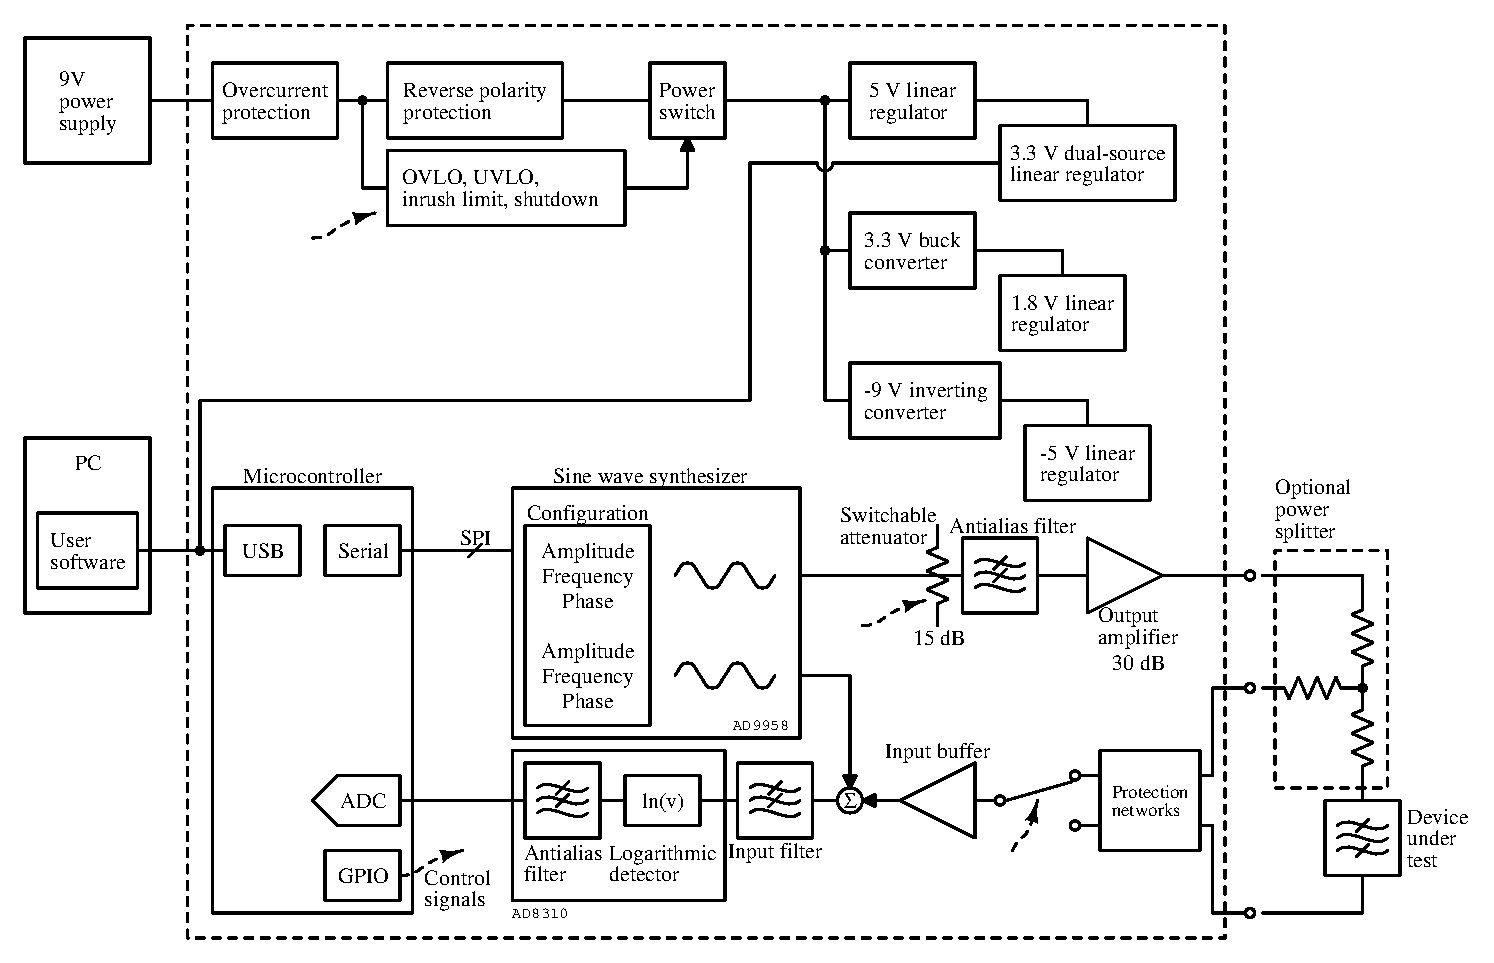
\includegraphics[width=6.5in]{blockdiagram}
\caption{Block diagram}
\label{fig:blockdiagram}
\end{figure}
\begin{multicols}{2}

\chapter{Theory of Operation}

This section contains a decription of the operation of the gain/phase analyzer.
Explanations range from simple and broad to very specific.
It is expected that the reader has an understanding of the basics of
gain/phase analysis itself, which is explained in the \hyperref[chap:intro]{Introduction
chapter}.

Also, it will be beneficial to look at the main system schematics when reading
through this section. Small pieces of the schematic are excerpted when helpful
in explaining their function, but are not always shown.

\section{Block Description}

The block diagram is shown in figure~\ref{fig:blockdiagram}. 


\section{Detailed Circuit Description}

\input{too/power}
\subsection{Synthesizer}

\schematicpage{3}{Synth}

In order to generate the test signals, a pair of sinusoids at anywhere from
1~kHz to above 150~MHz, the instrument uses a sophisticated
high-speed Direct Digital Synthesis (DDS) integrated circuit.

\begin{figure}[H]
\centering
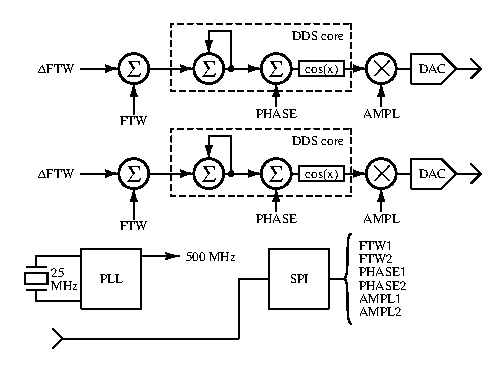
\includegraphics{dds}
\caption{DDS architecture}
\label{fig:dds}
\end{figure}

Figure~\ref{fig:dds} shows the internal architecture of the chip, somewhat
simplified from the version in the datasheet~\cite{ad9958}. In each of the two
independent waveform generators, a `frequency tuning word' (a 32-bit unsigned
integer) is repeatedly added to an accumulator at a rate of 500~MHz.
This causes the accumulator to increment, and overflow, at a higher rate for
higher tuning words. This sum is added to a phase offset, which allows each
signal to be independently offset from the other. This constantly incrementing
and resetting count is applied to a lookup table loaded with cosine values,
converting it from a digital ramp to a digital sinusoid. It is next multiplied
by an amplitude control value, and loaded into a digital-to-analog converter
(DAC) to generate the analog, sinusoidal waveform.

This integrated circuit is intended for radio applications. As such, it has
advanced features that this instrument does not require. It can be supplied
externally with a stable 500~MHz clock signal from a high quality
clock generator, but because we do not require such extreme stability, we
are instead using its internal Phase-Locked Loop (PLL) to multiply the clock
signal from a 25~MHz quartz crystal, \refdes{X1}, up to the full
internal clock frequency. Also, the device can generate modulated waveforms
using a 4-bit digital modulation input; these inputs are not used.

\subsection{Synthesizer Output Amplifiers}
\schematicpage{3}{Synth}

As is often the case with high-speed integrated circuits, the DDS chip has a
peculiar output system.

\begin{figure}[H]
\centering
\includegraphics{dds-output}
\caption{DDS output circuit}
\label{fig:ddsoutput}
\end{figure}

The outputs are symmetric current sinks, which pull up to 9.9~mA
down from AVDD (1.8~V), and the voltage that appears at these
outputs must not deviate by more than 500~mV from AVDD (or else
the signal will distort severely). The intended application is for these
to be connected to a center-tapped transformer, with the center tap connected
to AVDD. This is impractical due to the frequency range required: any
transformer with a high enough inductance to operate at 1~kHz has
too much parasitic capacitance to operate at 150~MHz. Instead,
a DC-coupled differential amplifier was used, with carefully designed
termination networks to provide the correct voltage range.

\begin{figure}[H]
\centering
\includegraphics{dds-outamp}
\caption{Output amplifier for synthesizer}
\label{fig:synthoutput}
\end{figure}

The 49.9~\Ohm{} resistors terminate the transmission line at the
source. The amplifier's inputs are relatively low impedance, so 53.6~\Ohm{}
resistors were used as load termination to provide a more accurate impedance when
placed in parallel with the differential amplifier.

Note that the input impedances of the two sides of the differential amplifier
are not equal. On the side entering the noninverting (`positive') input, the
impedance to ground is the sum of the two input resistors, or 720~\Ohm{}.
However, on the other side, the end of the feedback chain is not grounded, it is
a 180\dg{} phase-shifted copy of the input signal. The equivalent input impedance
here is only 360~\Ohm{}, and a more proper termination resistor there
would be 57.6~\Ohm{}. However, these transmission lines are very short,
and the difference in impedance does not make a significant difference. Using
two different resistors here would have increased the design complexity and cost,
and was deemed unnecessary. 
    

\subsection{Output System}
\schematicpage{4}{OutputAmp}

\subsubsection{Attenuator and Filter}
\subsubsection{Gain Stages and Termination}

\subsection{Input System}
\schematicpage{6}{InputFrontend}

\subsubsection{Protection}
\schematicpage{7}{Protection}

\subsubsection{Switching}

\schematicpage{8}{Switching}

It would not be practical for the analyzer to contain two independent input
subsystems to measure both inputs, as these systems are complex and expensive,
and there would be significant variation between the two. Instead, one input
subsystem is switched between two inputs. This switching is accomplished with a
pair of high-bandwidth SPST RF analog switches.

\begin{figure}[H]
\centering
\includegraphics{gaassw}
\caption{GaAs switch circuit}
\label{fig:gaassw}
\end{figure}

Figure~\ref{fig:gaassw} shows the internal circuit of the
switch~\cite{maswss0162}.  It is a simple circuit built from four gallium
arsenide (GaAs) FETs \footnote{The type of FET used is a relatively uncommon
    variant called a \emph{MESFET}, or MEtal-Semiconductor Field Effect
Transistor. This is a variant on the well known JFET, using a Schottky junction
instead of a PN junction. While uncommon in general, it is used often in GaAs
circuits due to the relative ease of constructing GaAs MESFETs.}.  These are
depletion-mode devices, so they are switched \emph{on} by applying zero volts
to the gate, and turned \emph{off} by applying a negative voltage, around
\Neg 5~V.  Switching on transistors \refdes{Q1} and \refdes{Q3} allows the
signal to pass through from the input to the output. Switching on transistors
\refdes{Q2} and \refdes{Q4} disconnects the input from the output, but also
\emph{terminates} the input (applies a $50\;\Omega$ resistance between the
input and ground). This is important to make sure that a disconnected input
does not cause signal reflections.

\begin{figure}[H]
\centering
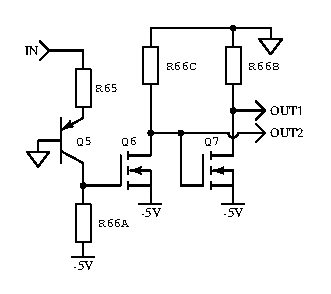
\includegraphics{gaasctl}
\caption{GaAs control circuit}
\label{fig:gaasctl}
\end{figure}

Figure~\ref{fig:gaasctl} is the control circuit for figure~\ref{fig:gaassw}.
When 0~V (a logic \emph{low}) is applied to the input from the
microcontroller, no current flows through \refdes{R65} or \refdes{R66A}.
This applies \Neg 5~V to \refdes{Q6}. Because \refdes{Q6}'s source is
connected to the \Neg 5~V rail instead of ground, the voltage between gate
and source ($V_{GS}$) is zero, and \refdes{Q6} is switched off.
This provides 0~V to one input of the GaAs switches. \refdes{Q7} acts
as an inverter, providing \Neg 5~V to the other GaAs switch input. The
dual switches have their inputs connected opposite each other, so this
switches one of them \emph{on} and the other \emph{off}.

When 3.3~V (a logic \emph{high}) is applied to the input from the
microcontroller, about 1.6~mA flows through \refdes{R65}. This
saturates \refdes{Q5}, applying about 0.7~V to \refdes{Q6}. As above,
$V_{GS}$ is the difference between this and the \Neg 5~V rail, or
5.7~V. \refdes{Q6} now switches on, and the two signals to the GaAs
switches swap places. This swaps the two switches, turning on the one that was
off, and turning off the one that was on.


\subsubsection{Buffer and Filter}
\schematicpage{9}{Buffer\_Filter}

\begin{figure}[H]
\centering
\missingfigure[figwidth=3in]{buffer}
\caption{Input buffer circuit}
\label{fig:buffer}
\end{figure}

Figure~\ref{fig:buffer} is the input signal buffer. \refdes{Q9} is a simple
emitter-follower (common collector) amplifier, providing isolation
between the input and further circuitry. \refdes{Q10} and \refdes{Q8} form
a current source to power it, in a feedback configuration providing
approximately $0.65\;\mr{V} / 30\;\Omega \approx 22\;\mr{mA}$.

The configuration of \refdes{R76} and \refdes{R77} sums together
the input signal and the phase reference signal, and this continues to the
input filter. \refdes{R75} combines with \refdes{R76} to properly
terminate the 50~\Ohm{} phase reference signal.

To lower the effect of external interference on the signals, a filter restricts
signals above the instrument's maximum operating frequency from continuing
past this point.

\subsubsection{Logarithmic Detector}
\schematicpage{10}{Detector}

\subsection{Microcontroller}
\schematicpage{13}{MPU}
\subsubsection{USB Communications}
\schematicpage{2}{Comm}




\section{Software Description}
\subsection{Signal Processing}
\subsubsection{Sampling}
\subsubsection{Null Search}
\subsubsection{Calibration}
\subsection{User Interface}



\end{multicols}

\newpage
\begin{landscape}
\chapter{Electrical parts}
\texttt{
\begin{longtable}{|l|l|l|l|l|}
\hline
\textbf{Reference} & \textbf{Manufacturer} & \textbf{Part Number} & \textbf{Line} & \textbf{Description} \\
\hline
\endhead
C1 &  &  & CAP MLCC 10nF 50V 10\% \ensuremath{\geq}X5R [0603] &  \\
\hline
C2 &  &  & CAP MLCC 10nF 50V 10\% \ensuremath{\geq}X5R [0603] &  \\
\hline
C3 &  &  & CAP MLCC 100nF 16V 10\% \ensuremath{\geq}X7R [0603] &  \\
\hline
C4 &  &  & CAP MLCC 10nF 50V 10\% \ensuremath{\geq}X5R [0603] &  \\
\hline
C5 &  &  & CAP MLCC 10\ensuremath{\mu}F 10V 10\% \ensuremath{\geq}X5R [0805] &  \\
\hline
C8 &  &  & CAP MLCC 100nF 16V 10\% \ensuremath{\geq}X7R [0603] &  \\
\hline
C9 &  &  & CAP MLCC 100nF 16V 10\% \ensuremath{\geq}X7R [0603] &  \\
\hline
C10 &  &  & CAP MLCC 100nF 16V 10\% \ensuremath{\geq}X7R [0603] &  \\
\hline
C11 &  &  & CAP MLCC 100nF 16V 10\% \ensuremath{\geq}X7R [0603] &  \\
\hline
C12 &  &  & CAP MLCC 100nF 16V 10\% \ensuremath{\geq}X7R [0603] &  \\
\hline
C13 &  &  & CAP MLCC 100nF 16V 10\% \ensuremath{\geq}X7R [0603] &  \\
\hline
C14 &  &  & CAP MLCC 15pF 50V 10\% C0G [0603] &  \\
\hline
C15 &  &  & CAP MLCC 15pF 50V 10\% C0G [0603] &  \\
\hline
C16 &  &  & CAP MLCC 100nF 16V 10\% \ensuremath{\geq}X7R [0603] &  \\
\hline
C17 &  &  & CAP MLCC 100nF 16V 10\% \ensuremath{\geq}X7R [0603] &  \\
\hline
C18 &  &  & CAP MLCC 100nF 16V 10\% \ensuremath{\geq}X7R [0603] &  \\
\hline
C19 &  &  & CAP MLCC 100nF 16V 10\% \ensuremath{\geq}X7R [0603] &  \\
\hline
C20 &  &  & CAP MLCC 100nF 16V 10\% \ensuremath{\geq}X7R [0603] &  \\
\hline
C21 &  &  & CAP MLCC 100nF 20V 10\% \ensuremath{\geq}X7R [0805] &  \\
\hline
C22 &  &  & CAP MLCC 100nF 16V 10\% \ensuremath{\geq}X7R [0603] &  \\
\hline
C23 &  &  & CAP MLCC 100nF 16V 10\% \ensuremath{\geq}X7R [0603] &  \\
\hline
C24 &  &  & CAP MLCC 100nF 20V 10\% \ensuremath{\geq}X7R [0805] &  \\
\hline
C25 &  &  & CAP MLCC 680pF 16V 5\% C0G [0603] &  \\
\hline
C26 &  &  & CAP MLCC 100nF 16V 10\% \ensuremath{\geq}X7R [0603] &  \\
\hline
C27 &  &  & CAP MLCC 100nF 16V 10\% \ensuremath{\geq}X7R [0603] &  \\
\hline
C28 &  &  & CAP MLCC 10\ensuremath{\mu}F 10V 10\% \ensuremath{\geq}X5R [0805] &  \\
\hline
C29 &  &  & CAP MLCC 10\ensuremath{\mu}F 10V 10\% \ensuremath{\geq}X5R [0805] &  \\
\hline
C30 &  &  & CAP MLCC 100nF 16V 10\% \ensuremath{\geq}X7R [0603] &  \\
\hline
C31 &  &  & CAP MLCC 100nF 16V 10\% \ensuremath{\geq}X7R [0603] &  \\
\hline
C32 &  &  & CAP MLCC 1nF 50V 10\% C0G [0603] &  \\
\hline
C33 &  &  & CAP MLCC 1nF 50V 10\% C0G [0603] &  \\
\hline
C34 &  &  & CAP MLCC 100nF 16V 10\% \ensuremath{\geq}X7R [0603] &  \\
\hline
C35 &  &  & CAP MLCC 100nF 16V 10\% \ensuremath{\geq}X7R [0603] &  \\
\hline
C36 &  &  & CAP MLCC 10\ensuremath{\mu}F 10V 10\% \ensuremath{\geq}X5R [0805] &  \\
\hline
C37 &  &  & CAP MLCC 10\ensuremath{\mu}F 10V 10\% \ensuremath{\geq}X5R [0805] &  \\
\hline
C38 &  &  & CAP MLCC 100nF 20V 10\% \ensuremath{\geq}X7R [0805] &  \\
\hline
C39 &  &  & CAP MLCC 100nF 20V 10\% \ensuremath{\geq}X7R [0805] &  \\
\hline
C40 &  &  & CAP MLCC 10\ensuremath{\mu}F 25V 10\% \ensuremath{\geq}X5R [1206] &  \\
\hline
C41 &  &  & CAP MLCC 10\ensuremath{\mu}F 25V 10\% \ensuremath{\geq}X5R [1206] &  \\
\hline
C43 & Murata & GRM1555C1H220GA01D & DIST DIGIKEY 490-6219-1-ND & CAP MLCC 22pF C0G [0402] \\
\hline
C44 & Murata & GRM1555C1H220GA01D & DIST DIGIKEY 490-6219-1-ND & CAP MLCC 22pF C0G [0402] \\
\hline
C45 & Samsung & CL10C1R5BB8NNNC & DIST DIGIKEY 1276-1656-1-ND & CAP MLCC 1.5pF C0G [0402] \\
\hline
C46 & Samsung & CL05C560JB5NNNC & DIST DIGIKEY 1276-1707-1-ND & CAP MLCC 56pF C0G [0402] \\
\hline
C47 & Samsung & CL05C4R7CB5NNNC & DIST DIGIKEY 1276-1703-1-ND & CAP MLCC 4.7pF C0G [0402] \\
\hline
C48 & Samsung & CL05C4R7CB5NNNC & DIST DIGIKEY 1276-1703-1-ND & CAP MLCC 4.7pF C0G [0402] \\
\hline
C49 & Samsung & CL05C560JB5NNNC & DIST DIGIKEY 1276-1707-1-ND & CAP MLCC 56pF C0G [0402] \\
\hline
C50 & Samsung & CL05C4R7CB5NNNC & DIST DIGIKEY 1276-1703-1-ND & CAP MLCC 4.7pF C0G [0402] \\
\hline
C51 & Murata & GRM1555C1H220GA01D & DIST DIGIKEY 490-6219-1-ND & CAP MLCC 22pF C0G [0402] \\
\hline
C52 & Murata & GRM1555C1H220GA01D & DIST DIGIKEY 490-6219-1-ND & CAP MLCC 22pF C0G [0402] \\
\hline
C53 &  &  & CAP MLCC 47\ensuremath{\mu}F 10V 20\% \ensuremath{\geq}X5R [1206] &  \\
\hline
C54 &  &  & CAP MLCC 1nF 50V 10\% C0G [0603] &  \\
\hline
C55 &  &  & CAP MLCC 100nF 20V 10\% \ensuremath{\geq}X7R [0805] &  \\
\hline
C56 &  &  & CAP MLCC 10nF 50V 10\% \ensuremath{\geq}X5R [0603] &  \\
\hline
C57 &  &  & CAP MLCC 1nF 50V 10\% C0G [0603] &  \\
\hline
C58 &  &  & CAP MLCC 1nF 50V 10\% C0G [0603] &  \\
\hline
C59 &  &  & CAP MLCC 100nF 16V 10\% \ensuremath{\geq}X7R [0603] &  \\
\hline
C60 & TDK & C1608C0G1H220F080AA & DIST DIGIKEY 445-5366-1-ND & CAP MLCC 22pF C0G [0402] \\
\hline
C61 & TDK & C1608C0G1H330F080AA & DIST DIGIKEY 445-7027-1-ND & CAP MLCC 33pF C0G [0402] \\
\hline
C62 & TDK & C1608C0G1H220F080AA & DIST DIGIKEY 445-5366-1-ND & CAP MLCC 22pF C0G [0402] \\
\hline
C63 &  &  & CAP MLCC 10nF 50V 10\% \ensuremath{\geq}X5R [0603] &  \\
\hline
C64 & TDK & C2012JB1H105K085AB & DIST DIGIKEY 445-11490-1-ND & CAP MLCC 1uF [0805] \\
\hline
C65 &  &  & CAP MLCC 10nF 50V 10\% \ensuremath{\geq}X5R [0603] &  \\
\hline
C66 & TDK & C2012JB1H105K085AB & DIST DIGIKEY 445-11490-1-ND & CAP MLCC 1uF [0805] \\
\hline
C67 &  &  & CAP MLCC 10nF 50V 10\% \ensuremath{\geq}X5R [0603] &  \\
\hline
C68 &  &  & CAP MLCC 100nF 16V 10\% \ensuremath{\geq}X7R [0603] &  \\
\hline
C69 &  &  & CAP MLCC 47\ensuremath{\mu}F 10V 20\% \ensuremath{\geq}X5R [1206] &  \\
\hline
C70 &  &  & CAP MLCC 220pF 16V 5\% C0G [0603] &  \\
\hline
C71 &  &  & CAP MLCC 330nF 50V 5\% \ensuremath{\geq}X7R [0603] &  \\
\hline
C72 &  &  & CAP MLCC 10nF 50V 10\% \ensuremath{\geq}X5R [0603] &  \\
\hline
C73 &  &  & CAP MLCC 100nF 20V 10\% \ensuremath{\geq}X7R [0805] &  \\
\hline
C74 &  &  & CAP MLCC 100nF 20V 10\% \ensuremath{\geq}X7R [0805] &  \\
\hline
C75 &  &  & CAP MLCC 10nF 50V 10\% \ensuremath{\geq}X5R [0603] &  \\
\hline
C76 & Panasonic & 16SVPC100M & DIST DIGIKEY P16468CT-ND & CAP ALU-POLY 100uF 16V \\
\hline
C77 & Panasonic & 16SVPC100M & DIST DIGIKEY P16468CT-ND & CAP ALU-POLY 100uF 16V \\
\hline
C78 &  &  & CAP MLCC 10nF 50V 10\% \ensuremath{\geq}X5R [0603] &  \\
\hline
C79 &  &  & CAP MLCC 10nF 50V 10\% \ensuremath{\geq}X5R [0603] &  \\
\hline
C80 &  &  & CAP MLCC 1nF 50V 10\% C0G [0603] &  \\
\hline
C81 &  &  & CAP MLCC 1nF 50V 10\% C0G [0603] &  \\
\hline
C82 & Panasonic & 16SVPC100M & DIST DIGIKEY P16468CT-ND & CAP ALU-POLY 100uF 16V \\
\hline
C83 & Panasonic & 16SVPC100M & DIST DIGIKEY P16468CT-ND & CAP ALU-POLY 100uF 16V \\
\hline
C84 &  &  & CAP MLCC 1\ensuremath{\mu}F 16V 10\% \ensuremath{\geq}X5R [1206] &  \\
\hline
C85 &  &  & CAP MLCC 1\ensuremath{\mu}F 16V 10\% \ensuremath{\geq}X5R [1206] &  \\
\hline
C86 &  &  & CAP MLCC 1\ensuremath{\mu}F 16V 10\% \ensuremath{\geq}X5R [1206] &  \\
\hline
C87 &  &  & CAP MLCC 1\ensuremath{\mu}F 16V 10\% \ensuremath{\geq}X5R [1206] &  \\
\hline
C88 &  &  & CAP MLCC 1\ensuremath{\mu}F 10V 10\% \ensuremath{\geq}X5R [0805] &  \\
\hline
C89 &  &  & CAP MLCC 1\ensuremath{\mu}F 16V 10\% \ensuremath{\geq}X5R [1206] &  \\
\hline
C90 &  &  & CAP MLCC 10\ensuremath{\mu}F 10V 10\% \ensuremath{\geq}X5R [0805] &  \\
\hline
C91 &  &  & CAP MLCC 10\ensuremath{\mu}F 10V 10\% \ensuremath{\geq}X5R [0805] &  \\
\hline
C92 &  &  & CAP MLCC 22\ensuremath{\mu}F 6V 10\% \ensuremath{\geq}X5R [0805] &  \\
\hline
C93 &  &  & CAP MLCC 1\ensuremath{\mu}F 10V 10\% \ensuremath{\geq}X5R [0805] &  \\
\hline
C97 &  &  & CAP MLCC 100nF 16V 10\% \ensuremath{\geq}X7R [0603] &  \\
\hline
C98 &  &  & CAP MLCC 100nF 16V 10\% \ensuremath{\geq}X7R [0603] &  \\
\hline
C100 &  &  & CAP MLCC 100nF 16V 10\% \ensuremath{\geq}X7R [0603] &  \\
\hline
C101 &  &  & CAP MLCC 100nF 16V 10\% \ensuremath{\geq}X7R [0603] &  \\
\hline
C102 &  &  & CAP MLCC 100nF 16V 10\% \ensuremath{\geq}X7R [0603] &  \\
\hline
C103 &  &  & CAP MLCC 100nF 16V 10\% \ensuremath{\geq}X7R [0603] &  \\
\hline
C104 &  &  & CAP MLCC 100nF 16V 10\% \ensuremath{\geq}X7R [0603] &  \\
\hline
C105 &  &  & CAP MLCC 100nF 16V 10\% \ensuremath{\geq}X7R [0603] &  \\
\hline
C106 &  &  & CAP MLCC 100nF 16V 10\% \ensuremath{\geq}X7R [0603] &  \\
\hline
C107 &  &  & CAP MLCC 10\ensuremath{\mu}F 10V 10\% \ensuremath{\geq}X5R [0805] &  \\
\hline
C108 &  &  & CAP MLCC 10\ensuremath{\mu}F 10V 10\% \ensuremath{\geq}X5R [0805] &  \\
\hline
C109 &  &  & CAP MLCC 1\ensuremath{\mu}F 10V 10\% \ensuremath{\geq}X5R [0805] &  \\
\hline
C110 &  &  & CAP MLCC 15pF 50V 10\% C0G [0603] &  \\
\hline
C111 &  &  & CAP MLCC 15pF 50V 10\% C0G [0603] &  \\
\hline
D3 &  & MMBD4148 & SEMI GENERIC MMBD4148 &  \\
\hline
D4 &  & MMBD4148 & SEMI GENERIC MMBD4148 &  \\
\hline
D5 &  & MMBD4148 & SEMI GENERIC MMBD4148 &  \\
\hline
D6 &  & MMBD4148 & SEMI GENERIC MMBD4148 &  \\
\hline
D7 &  & MBR0540 & SEMI GENERIC MBR0540 &  \\
\hline
D8 &  & MBR0540 & SEMI GENERIC MBR0540 &  \\
\hline
DS1 &  & LED RED [3mm] & SEMI GENERIC LED RED [3mm] &  \\
\hline
DS2 &  & LED RED [0603] & SEMI GENERIC LED RED [0603] &  \\
\hline
DS3 &  & LED RED [0603] & SEMI GENERIC LED RED [0603] &  \\
\hline
DS4 &  & LED RED [0603] & SEMI GENERIC LED RED [0603] &  \\
\hline
DS5 &  & LED RED [0603] & SEMI GENERIC LED RED [0603] &  \\
\hline
DS6 &  & LED RED [0603] & SEMI GENERIC LED RED [0603] &  \\
\hline
DS7 &  & LED RED [0603] & SEMI GENERIC LED RED [0603] &  \\
\hline
DS8 &  & LED RED [0603] & SEMI GENERIC LED RED [0603] &  \\
\hline
DS9 &  & LED RED [0603] & SEMI GENERIC LED RED [0603] &  \\
\hline
DS10 &  & LED RED [0603] & SEMI GENERIC LED RED [0603] &  \\
\hline
DS11 &  & LED RED [0603] & SEMI GENERIC LED RED [0603] &  \\
\hline
DZ1 & ONSEMI & 1SMA5914BT3G & SEMI ONSEMI 1SMA5914BT3G &  \\
\hline
DZ2 & LITTELFUSE & SP0503BAHT & SEMI LITTELFUSE SP0503BAHT &  \\
\hline
DZ3 & ONSEMI & ESD9L5.0ST5G & SEMI ONSEMI ESD9L5.0ST5G &  \\
\hline
DZ4 & ONSEMI & ESD9L5.0ST5G & SEMI ONSEMI ESD9L5.0ST5G &  \\
\hline
DZ5 &  & BZX84C2V7 & SEMI GENERIC BZX84C2V7 &  \\
\hline
DZ6 &  & BZX84C2V7 & SEMI GENERIC BZX84C2V7 &  \\
\hline
DZ7 & ONSEMI & ESD9L5.0ST5G & SEMI ONSEMI ESD9L5.0ST5G &  \\
\hline
DZ8 & ONSEMI & ESD9L5.0ST5G & SEMI ONSEMI ESD9L5.0ST5G &  \\
\hline
DZ9 &  & BZX84C3V9 & SEMI GENERIC BZX84C3V9 &  \\
\hline
DZ10 &  & BZX84C10 & SEMI GENERIC BZX84C10 &  \\
\hline
E1 & Laird & HZ0805B222R-10 & DIST DIGIKEY 240-2562-1-ND & FERRITE CHIP 2.2k @ 100MHz [0805] \\
\hline
E2 & Laird & HZ0805B222R-10 & DIST DIGIKEY 240-2562-1-ND & FERRITE CHIP 2.2k @ 100MHz [0805] \\
\hline
E5 & Bourns & MZ1608-102Y & DIST DIGIKEY MZ1608-102YCT-ND & FERRITE CHIP 1k @ 100MHz [0603] \\
\hline
J1 & CUI & PJ-037A & DIST DIGIKEY CP-037A-ND & CONN BARREL 2x6.5MM \\
\hline
J2 & TE & 5-1814400-1 & DIST DIGIKEY A97593-ND & CONN SMA RIGHTANGLE FEMALE \\
\hline
J3 & TE & 5-1814400-1 & DIST DIGIKEY A97593-ND & CONN SMA RIGHTANGLE FEMALE \\
\hline
J4 & TE & 5-1814400-1 & DIST DIGIKEY A97593-ND & CONN SMA RIGHTANGLE FEMALE \\
\hline
J6 & FCI & 10118194-0001LF & DIST DIGIKEY 609-4618-1-ND & CONN USB MICRO-B FEMALE \\
\hline
J8 & ONSHORE & 302-S201 & DIST DIGIKEY ED10524-ND & HEADER 2x10 100MIL SHROUDED \\
\hline
L1 & Samsung & CIH05T56NJNC & DIST DIGIKEY 1276-6281-1-ND & IND CHIP 56nH \\
\hline
L2 & Samsung & CIH05T47NJNC & DIST DIGIKEY 1276-6280-1-ND & IND CHIP 47nH \\
\hline
L3 & Samsung & CIH05T47NJNC & DIST DIGIKEY 1276-6280-1-ND & IND CHIP 47nH \\
\hline
L4 & Panasonic & ELJ-RF39NGFB & DIST DIGIKEY PCD1917CT-ND & IND CHIP 39nH \\
\hline
L5 & Panasonic & ELJ-RF39NGFB & DIST DIGIKEY PCD1917CT-ND & IND CHIP 39nH \\
\hline
L6 & Bourns & RLB0914-221KL & DIST DIGIKEY RLB0914-221KL-ND & IND WOUND 220uH 700mA \\
\hline
L7 & Bourns & RLB0914-221KL & DIST DIGIKEY RLB0914-221KL-ND & IND WOUND 220uH 700mA \\
\hline
L8 & TDK & MLZ2012M4R7HT000 & DIST DIGIKEY 445-8659-1-ND & IND CHIP 4.7uH 300mA [0805] \\
\hline
L9 & TDK & MLZ2012M4R7HT000 & DIST DIGIKEY 445-8659-1-ND & IND CHIP 4.7uH 300mA [0805] \\
\hline
L10 & TDK & MLZ2012M4R7HT000 & DIST DIGIKEY 445-8659-1-ND & IND CHIP 4.7uH 300mA [0805] \\
\hline
MP5 & Laird & BMI-S-203F; BMI-S-203-C & DIST DIGIKEY 903-1052-1-ND; & RF SHIELD TWO-PIECE \\
\hline
Q1 & IRF & IRLML6402 & SEMI IRF IRLML6402 &  \\
\hline
Q2 &  & MMBT3906 & SEMI GENERIC MMBT3906 &  \\
\hline
Q3 &  & 2N7002 & SEMI GENERIC 2N7002 &  \\
\hline
Q4 &  & 2N7002 & SEMI GENERIC 2N7002 &  \\
\hline
Q5 &  & MMBT3906 & SEMI GENERIC MMBT3906 &  \\
\hline
Q6 &  & 2N7002 & SEMI GENERIC 2N7002 &  \\
\hline
Q7 &  & 2N7002 & SEMI GENERIC 2N7002 &  \\
\hline
Q8 &  & MMBT3904 & SEMI GENERIC MMBT3904 &  \\
\hline
Q9 & NXP & BFR540 & SEMI NXP BFR540 &  \\
\hline
Q10 & NXP & BFR540 & SEMI NXP BFR540 &  \\
\hline
Q11 &  & MMBT3904 & SEMI GENERIC MMBT3904 &  \\
\hline
Q12 &  & MMBT3906 & SEMI GENERIC MMBT3906 &  \\
\hline
Q13 & IRF & IRLML6402 & SEMI IRF IRLML6402 &  \\
\hline
Q14 & AOS & AOD417 & SEMI AOS AOD417 &  \\
\hline
Q15 &  & MMBT3904 & SEMI GENERIC MMBT3904 &  \\
\hline
Q16 &  & MMBT3904 & SEMI GENERIC MMBT3904 &  \\
\hline
Q17 &  & PZT2907A & SEMI GENERIC PZT2907A &  \\
\hline
Q18 &  & PZT2907A & SEMI GENERIC PZT2907A &  \\
\hline
Q19 &  & MMBT3904 & SEMI GENERIC MMBT3904 &  \\
\hline
Q20 &  & MMBT3904 & SEMI GENERIC MMBT3904 &  \\
\hline
R1 &  &  & RES SMD 3.3k 5\% [0603] &  \\
\hline
R2 &  &  & RES SMD 1.6k 1\% [0603] &  \\
\hline
R3 &  &  & RES SMD 1.6k 1\% [0603] &  \\
\hline
R4 &  &  & RES SMD 3.3k 5\% [0603] &  \\
\hline
R5 &  &  & RES SMD 1.6k 1\% [0603] &  \\
\hline
R6 &  &  & RES SMD 1.6k 1\% [0603] &  \\
\hline
R7 &  &  & RES SMD 1.6k 1\% [0603] &  \\
\hline
R8 &  &  & RES SMD 3.3k 5\% [0603] &  \\
\hline
R9 &  &  & RES SMD 3.3k 5\% [0603] &  \\
\hline
R10 & Bel Fuse & 0ZCJ0005FF2E & DIST DIGIKEY 507-1793-1-ND & PPTC 50mA/150mA 60V [1206] \\
\hline
R11 & Bel Fuse & 0ZCJ0005FF2E & DIST DIGIKEY 507-1793-1-ND & PPTC 50mA/150mA 60V [1206] \\
\hline
R12 & Bel Fuse & 0ZCJ0005FF2E & DIST DIGIKEY 507-1793-1-ND & PPTC 50mA/150mA 60V [1206] \\
\hline
R13 &  &  & RES SMD 1M 5\% [0603] &  \\
\hline
R14 &  &  & RES SMD 30 1\% [0603] &  \\
\hline
R15 &  &  & RES SMD 30 1\% [0603] &  \\
\hline
R16 &  &  & RES SMD 1M 5\% [0603] &  \\
\hline
R17 &  &  & RES SMD 1M 5\% [0603] &  \\
\hline
R18 &  &  & RES SMD 49.9 1\% [0603] &  \\
\hline
R19 &  &  & RES SMD 1.91k 1\% [0603] &  \\
\hline
R21 &  &  & RES SMD 49.9 1\% [0603] &  \\
\hline
R22 &  &  & RES SMD 49.9 1\% [0603] &  \\
\hline
R23 &  &  & RES SMD 49.9 1\% [0603] &  \\
\hline
R24 &  &  & RES SMD 53.6 1\% [0603] &  \\
\hline
R25 &  &  & RES SMD 53.6 1\% [0603] &  \\
\hline
R26 &  &  & RES SMD 53.6 1\% [0603] &  \\
\hline
R27 &  &  & RES SMD 53.6 1\% [0603] &  \\
\hline
R28 &  &  & RES SMD 360 1\% [0603] &  \\
\hline
R29 &  &  & RES SMD 360 1\% [0603] &  \\
\hline
R30 &  &  & RES SMD 360 1\% [0603] &  \\
\hline
R31 &  &  & RES SMD 360 1\% [0603] &  \\
\hline
R32 &  &  & RES SMD 360 1\% [0603] &  \\
\hline
R33 &  &  & RES SMD 360 1\% [0603] &  \\
\hline
R34 &  &  & RES SMD 360 1\% [0603] &  \\
\hline
R35 &  &  & RES SMD 360 1\% [0603] &  \\
\hline
R36 &  &  & RES SMD 1.91k 1\% [0603] &  \\
\hline
R37 &  &  & RES SMD 1.91k 1\% [0603] &  \\
\hline
R38 &  &  & RES SMD 49.9 1\% [0603] &  \\
\hline
R39 &  &  & RES SMD 49.9 1\% [0603] &  \\
\hline
R40 &  &  & RES SMD 1.6k 1\% [0603] &  \\
\hline
R41 & Yageo & YC164-JR-0710KL & DIST DIGIKEY YC164J-10KCT-ND & RESPACK SMD 10k 5\% [4x0603] \\
\hline
R42 &  &  & RES SMD 200 1\% [0603] &  \\
\hline
R43 &  &  & RES SMD 200 1\% [0603] &  \\
\hline
R45 &  &  & RES SMD 30 1\% [0603] &  \\
\hline
R46 &  &  & RES SMD 49.9 1\% [0603] &  \\
\hline
R47 &  &  & RES SMD 150 1\% [0603] &  \\
\hline
R48 &  &  & RES SMD 750 1\% [0603] &  \\
\hline
R49 &  &  & RES SMD 150 1\% [0603] &  \\
\hline
R50 &  &  & RES SMD 33 1\% [0603] &  \\
\hline
R51 &  &  & RES SMD 33 1\% [0603] &  \\
\hline
R52 &  &  & RES SMD 33 1\% [0603] &  \\
\hline
R53 &  &  & RES SMD 33 1\% [0603] &  \\
\hline
R54 &  &  & RES SMD 33 1\% [0603] &  \\
\hline
R55 &  &  & RES SMD 33 1\% [0603] &  \\
\hline
R56 &  &  & RES SMD 49.9 1\% [0603] &  \\
\hline
R57 &  &  & RES SMD 1.6k 1\% [0603] &  \\
\hline
R58 &  &  & RES SMD 1.6k 1\% [0603] &  \\
\hline
R59 &  &  & RES SMD 3.3 10\% [0603] &  \\
\hline
R60 &  &  & RES SMD 750 1\% [0603] &  \\
\hline
R61 &  &  & RES SMD 750 1\% [0603] &  \\
\hline
R62 &  &  & RES SMD 1.6k 1\% [0603] &  \\
\hline
R63 &  &  & RES SMD 1.6k 1\% [0603] &  \\
\hline
R64 &  &  & RES SMD 3.3 10\% [0603] &  \\
\hline
R65 &  &  & RES SMD 1.6k 1\% [0603] &  \\
\hline
R66 & Yageo & YC164-JR-0710KL & DIST DIGIKEY YC164J-10KCT-ND & RESPACK SMD 10k 5\% [4x0603] \\
\hline
R67 &  &  & RES SMD 200 1\% [0603] &  \\
\hline
R68 &  &  & RES SMD 200 1\% [0603] &  \\
\hline
R69 &  &  & RES SMD 200 1\% [0603] &  \\
\hline
R70 &  &  & RES SMD 200 1\% [0603] &  \\
\hline
R71 &  &  & RES SMD 200 1\% [0603] &  \\
\hline
R72 &  &  & RES SMD 200 1\% [0603] &  \\
\hline
R73 &  &  & RES SMD 1.6k 1\% [0603] &  \\
\hline
R74 &  &  & RES SMD 30 1\% [0603] &  \\
\hline
R75 &  &  & RES SMD 100 1\% [0603] &  \\
\hline
R76 &  &  & RES SMD 100 1\% [0603] &  \\
\hline
R77 &  &  & RES SMD 100 1\% [0603] &  \\
\hline
R78 &  &  & RES SMD 3.3k 5\% [0603] &  \\
\hline
R79 &  &  & RES SMD 53.6 1\% [0603] &  \\
\hline
R80 &  &  & RES SMD 49.9 1\% [0603] &  \\
\hline
R81 & BelFuse & 0ZCJ0035AF2E & DIST DIGIKEY 507-1801-1-ND & PPTC 350mA/750mA 30V [1206] \\
\hline
R82 &  &  & RES SMD 3.3k 5\% [0603] &  \\
\hline
R83 & Yageo & YC164-JR-0710KL & DIST DIGIKEY YC164J-10KCT-ND & RESPACK SMD 10k 5\% [4x0603] \\
\hline
R84 & Yageo & YC164-JR-0710KL & DIST DIGIKEY YC164J-10KCT-ND & RESPACK SMD 10k 5\% [4x0603] \\
\hline
R85 & Yageo & YC164-JR-0710KL & DIST DIGIKEY YC164J-10KCT-ND & RESPACK SMD 10k 5\% [4x0603] \\
\hline
R86 &  &  & RES SMD 3.3k 5\% [0603] &  \\
\hline
R87 &  &  & RES SMD 1M 5\% [0603] &  \\
\hline
R88 &  &  & RES SMD 1M 5\% [0603] &  \\
\hline
R89 &  &  & RES SMD 3.3k 5\% [0603] &  \\
\hline
R90 &  &  & RES SMD 3.3k 5\% [0603] &  \\
\hline
R91 &  &  & RES SMD 1.6k 1\% [0603] &  \\
\hline
R92 &  &  & RES SMD 750 1\% [0603] &  \\
\hline
R93 &  &  & RES SMD 1.6k 1\% [0603] &  \\
\hline
R94 &  &  & RES SMD 750 1\% [0603] &  \\
\hline
R95 &  &  & RES SMD 1 5\% [1210] &  \\
\hline
R96 &  &  & RES SMD 1 5\% [1210] &  \\
\hline
R97 & BelFuse & 0ZCJ0010FF2E & DIST DIGIKEY 507-1794-1-ND & PPTC 100mA/250mA 60V [1206] \\
\hline
R98 &  &  & RES SMD 3.3 10\% [0603] &  \\
\hline
R99 &  &  & RES SMD 3.3 10\% [0603] &  \\
\hline
R102 &  &  & RES SMD 3.3k 5\% [0603] &  \\
\hline
R103 &  &  & RES SMD 3.3k 5\% [0603] &  \\
\hline
R104 &  &  & RES SMD 3.3k 5\% [0603] &  \\
\hline
R105 &  &  & RES SMD 3.3k 5\% [0603] &  \\
\hline
R106 &  &  & RES SMD 1k 5\% [0603] &  \\
\hline
R107 &  &  & RES SMD 1k 5\% [0603] &  \\
\hline
R108 &  &  & RES SMD 1k 5\% [0603] &  \\
\hline
R109 &  &  & RES SMD 1k 5\% [0603] &  \\
\hline
R110 &  &  & RES SMD 200 1\% [0603] &  \\
\hline
R111 &  &  & RES SMD 3.3k 5\% [0603] &  \\
\hline
R112 &  &  & RES SMD 200 1\% [0603] &  \\
\hline
R113 &  &  & RES SMD 200 1\% [0603] &  \\
\hline
R114 &  &  & RES SMD 200 1\% [0603] &  \\
\hline
R115 &  &  & RES SMD 200 1\% [0603] &  \\
\hline
R116 &  &  & RES SMD 200 1\% [0603] &  \\
\hline
R117 &  &  & RES SMD 360 1\% [0603] &  \\
\hline
U2 & TI & LMH6714MF & IC TI LMH6714MF &  \\
\hline
U3 & ADI & AD9958BCPZ & IC ADI AD9958BCPZ &  \\
\hline
U4 & TI & LMH6714MF & IC TI LMH6714MF &  \\
\hline
U5 & ADI & AD8000YRDZ & IC ADI AD8000YRDZ &  \\
\hline
U6 & TI & THS3001IDGN & IC TI THS3001IDGN &  \\
\hline
U7 & MACOM & MAADSS0008 & IC MACOM MAADSS0008 &  \\
\hline
U8 & MACOM & MASWSS0162 & IC MACOM MASWSS0162 &  \\
\hline
U9 & MACOM & MASWSS0162 & IC MACOM MASWSS0162 &  \\
\hline
U10 & ADI & AD8310ARMZ & IC ADI AD8310ARMZ &  \\
\hline
U11 & TI & TL431AIDBZ & IC TI TL431AIDBZ &  \\
\hline
U12 &  & LM393M & IC GENERIC LM393M &  \\
\hline
U13 & ST & L78M05CDT & IC ST L78M05CDT &  \\
\hline
U14 & ONSEMI & MC79M05CDTG & IC ONSEMI MC79M05CDTG &  \\
\hline
U15 & DIODES & AZ1117CH-1.8TRG1 & IC DIODES AZ1117CH-1.8TRG1 &  \\
\hline
U16 & MICROCHIP & MCP1700T-3302E/TT & IC MICROCHIP MCP1700T-3302E/TT &  \\
\hline
U18 & ATMEL & ATSAM4S16CA-AU & IC ATMEL ATSAM4S16CA-AU &  \\
\hline
X1 & TXC & 9C-25.000MEEJ-T & DIST DIGIKEY 887-1283-1-ND & CRYSTAL 25MHz 18pF 10PPM \\
\hline
X2 & Abracon & ABLS-12.000MHZ-B4-T & DIST DIGIKEY 535-10218-1-ND & CRYSTAL 12MHz 18pF \\
\hline
\end{longtable}

}
\end{landscape}

\newpage
\chapter{Full schematics}
The following pages contain schematics exported directly from the CAD software.
While they are documented, it is intended that readers will first familiarize
themselves with the workings of the circuits by reading through the
\hyperref[chap:too]{Theory of Operation}.
\includepdf[landscape=true,pages=-,link]{schematic.pdf}
\newpage
\begin{thebibliography}{9}

\bibitem{aod417}
Alpha \& Omega Semiconductor, ``AOD417 P-Channel Enhancement Mode Field Effect Transistor,''
AOD417 datasheet, 2008. \url{http://aosmd.com/pdfs/datasheet/AOD417.pdf}

\bibitem{tranckts-sawtooth}
S. W. Amos and M. James, ``Sawtooth generators,'' in
\emph{Principles of Transistor Circuits}, 9th ed. Oxford: Newnes, 2003, ch. 14, pp. 281--292.

\bibitem{ad9958}
Analog Devices, Inc., ``2-Channel, 500 MSPS DDS with 10-Bit DACs,'' AD9958 datasheet,
April 2013 [Revision B].
\url{http://www.analog.com/media/cn/technical-documentation/data-sheets/AD9958.pdf}

\bibitem{az1117c}
Diodes Incorporated, ``Low Dropout Linear Regulator,'' AZ1117C datasheet,
October 2014 [Revision 3--2].
\url{http://www.diodes.com/datasheets/AZ1117C.pdf}

\bibitem{aoe-vreg}
P. Horowitz and W. Hill, ``Voltage regulators and power circuits,'' in
\emph{The Art of Electronics}, 2nd ed. Cambridge: Cambridge, 1989, ch. 6, pp. 307--389.

\bibitem{maswss0162}
M/A-COM Technology, ``GaAs SPST Switch,'' MASWSS0162 datasheet [Revision V3].
\url{http://cdn.macom.com/DataSheets/MASWSS0162.pdf}

\bibitem{mcp1700}
Microchip Technology, ``Low Quiescent Current LDO,'' MCP1700 datasheet,
October 2013 [Revision C].
\url{http://ww1.microchip.com/downloads/en/DeviceDoc/20001826C.pdf}

\bibitem{mc79m00}
ON Semiconductor, ``500 mA Negative Voltage Regulators,'' MC79M00 series datasheet,
July 2013 [Revision 15].
\url{http://www.onsemi.com/pub_link/Collateral/MC79M00-D.PDF}.

\bibitem{l78m05}
STMicroelectronics, ``Precision 500 mA regulators,'' L78M datasheet, June 2014 [Revision 20].
\url{http://www.st.com/web/en/resource/technical/document/datasheet/CD00000447.pdf}

\bibitem{tl431}
Texas Instruments, ``TL43xx Precision Programmable Reference,''
TL431 datasheet, Aug. 2004 [Revised Jan. 2015]. \url{http://www.ti.com/lit/ds/symlink/tl431.pdf}

\bibitem{buckinv}
J. Tucker, ``Using a buck converter in an inverting buck-boost topology,''
\emph{Analog Applications Journal}, Texas Instruments, fourth quarter 2007, pp. 16--19.
\url{http://www.ti.com/lit/an/slyt286/slyt286.pdf}
\end{thebibliography}


\end{document}
